% RFT Publication-Quality Figures - LaTeX/TikZ/PGFPlots
% Compile with pdflatex
\documentclass[border=5pt]{standalone}
\usepackage{tikz}
\usepackage{pgfplots}
\usepackage{amsmath}
\usepackage{xcolor}

\pgfplotsset{compat=1.18}
\usepgfplotslibrary{groupplots}

% Define colors
\definecolor{rftcolor}{RGB}{231,76,60}
\definecolor{fftcolor}{RGB}{52,152,219}
\definecolor{dctcolor}{RGB}{46,204,113}
\definecolor{hadcolor}{RGB}{243,156,18}

\begin{document}

%% Figure 1: Unitarity Error Comparison
\begin{tikzpicture}
\begin{axis}[
    width=12cm,
    height=8cm,
    xlabel={Transform Size $N$},
    ylabel={Round-trip Error (relative)},
    title={\textbf{Unitarity Error: RFT vs FFT}},
    legend pos=north west,
    legend style={draw=black, fill=white, font=\small},
    grid=both,
    minor grid style={gray!25},
    major grid style={gray!50},
    xmode=log,
    ymode=log,
    log basis x=2,
    xtick={8,16,32,64,128,256,512,1024},
    xticklabels={8,16,32,64,128,256,512,1024},
    xmin=8, xmax=1024,
    ymin=1e-17, ymax=1e-14,
    mark size=3pt,
    line width=1.5pt,
]

% RFT data
\addplot[color=rftcolor, mark=o] table {figures/latex_data/unitarity_data.dat};
\addlegendentry{RFT ($\Phi$-RFT)}

% FFT data
\addplot[color=fftcolor, mark=square] table[x index=0, y index=2] {figures/latex_data/unitarity_data.dat};
\addlegendentry{FFT}

% Machine precision reference
\addplot[color=red, dashed, line width=1pt, domain=8:1024, samples=2] {1e-15};
\addlegendentry{Machine precision}

\end{axis}
\end{tikzpicture}

\vspace{1cm}

%% Figure 2: Performance Benchmark
\begin{tikzpicture}
\begin{semilogxaxis}[
    width=12cm,
    height=8cm,
    xlabel={Transform Size $N$},
    ylabel={Execution Time (ms)},
    title={\textbf{Computational Performance Comparison}},
    legend pos=north west,
    legend style={draw=black, fill=white, font=\small},
    grid=both,
    minor grid style={gray!25},
    major grid style={gray!50},
    log basis x=2,
    xtick={64,128,256,512,1024},
    xticklabels={64,128,256,512,1024},
    xmin=64, xmax=1024,
    mark size=3pt,
    line width=1.5pt,
]

% RFT data (convert to ms)
\addplot[color=rftcolor, mark=o] table[x index=0, y expr=\thisrow{1}*1000] {figures/latex_data/performance_data.dat};
\addlegendentry{RFT ($\Phi$-RFT)}

% FFT data
\addplot[color=fftcolor, mark=square] table[x index=0, y expr=\thisrow{2}*1000] {figures/latex_data/performance_data.dat};
\addlegendentry{FFT}

% DCT data
\addplot[color=dctcolor, mark=triangle] table[x index=0, y expr=\thisrow{3}*1000] {figures/latex_data/performance_data.dat};
\addlegendentry{DCT}

\end{semilogxaxis}
\end{tikzpicture}

\vspace{1cm}

%% Figure 3: Phase Structure Diagram
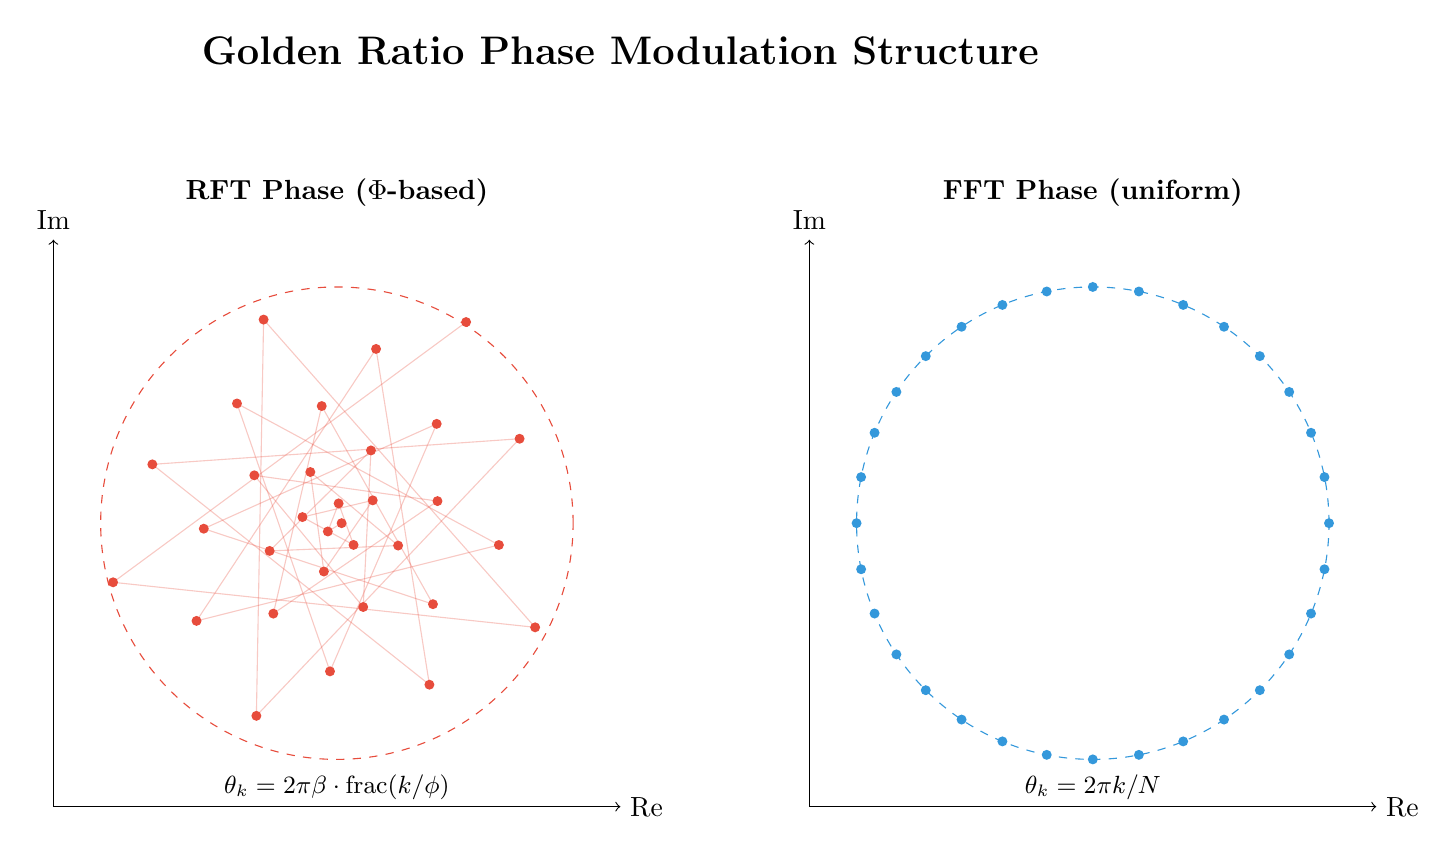
\begin{tikzpicture}[scale=1.2]
    % Title
    \node[font=\Large\bfseries] at (6, 8) {Golden Ratio Phase Modulation Structure};
    
    % RFT Phase spiral
    \begin{scope}[shift={(0,0)}]
        \node[font=\bfseries] at (3, 6.5) {RFT Phase ($\Phi$-based)};
        \draw[->] (0,0) -- (6,0) node[right] {Re};
        \draw[->] (0,0) -- (0,6) node[above] {Im};
        
        % Draw spiral based on golden ratio
        \foreach \k in {0,1,...,31} {
            \pgfmathsetmacro{\theta}{360*(\k/1.618034)}
            \pgfmathsetmacro{\r}{0.05 + 0.08*\k}
            \pgfmathsetmacro{\x}{\r*cos(\theta)}
            \pgfmathsetmacro{\y}{\r*sin(\theta)}
            \fill[rftcolor] (3+\x, 3+\y) circle (1.5pt);
            \ifnum\k>0
                \pgfmathsetmacro{\thetaprev}{360*((\k-1)/1.618034)}
                \pgfmathsetmacro{\rprev}{0.05 + 0.08*(\k-1)}
                \pgfmathsetmacro{\xprev}{\rprev*cos(\thetaprev)}
                \pgfmathsetmacro{\yprev}{\rprev*sin(\thetaprev)}
                \draw[rftcolor, opacity=0.3] (3+\xprev, 3+\yprev) -- (3+\x, 3+\y);
            \fi
        }
        \draw[rftcolor, dashed] (3,3) circle (2.5);
        \node[font=\small] at (3, 0.2) {$\theta_k = 2\pi \beta \cdot \text{frac}(k/\phi)$};
    \end{scope}
    
    % FFT Phase regular
    \begin{scope}[shift={(8,0)}]
        \node[font=\bfseries] at (3, 6.5) {FFT Phase (uniform)};
        \draw[->] (0,0) -- (6,0) node[right] {Re};
        \draw[->] (0,0) -- (0,6) node[above] {Im};
        
        % Draw uniform circle
        \foreach \k in {0,1,...,31} {
            \pgfmathsetmacro{\theta}{360*\k/32}
            \pgfmathsetmacro{\x}{2.5*cos(\theta)}
            \pgfmathsetmacro{\y}{2.5*sin(\theta)}
            \fill[fftcolor] (3+\x, 3+\y) circle (1.5pt);
        }
        \draw[fftcolor, dashed] (3,3) circle (2.5);
        \node[font=\small] at (3, 0.2) {$\theta_k = 2\pi k/N$};
    \end{scope}
\end{tikzpicture}

\vspace{1cm}

%% Figure 4: Transform Matrix Structure
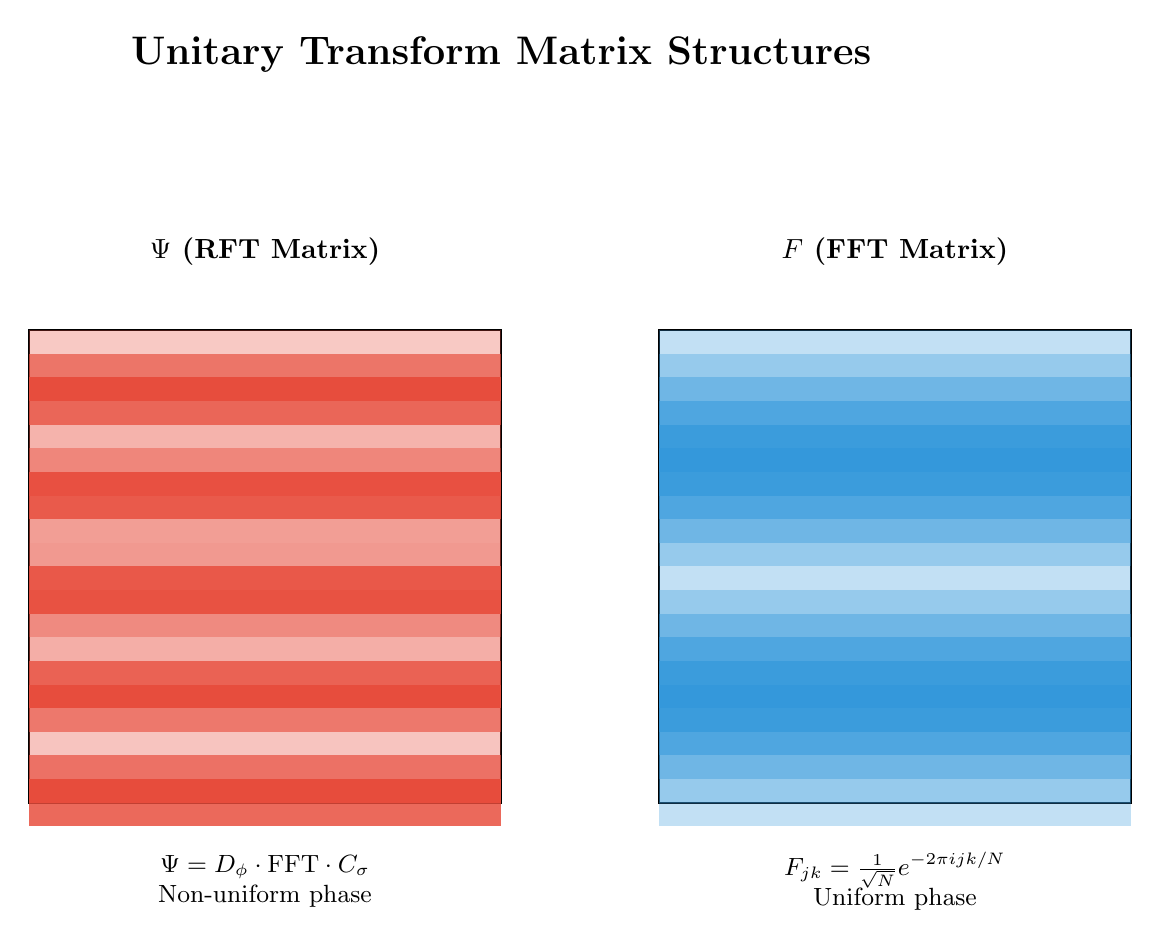
\begin{tikzpicture}
    \node[font=\Large\bfseries] at (6, 0.5) {Unitary Transform Matrix Structures};
    
    % RFT Matrix (symbolic)
    \begin{scope}[shift={(0,-2)}]
        \node[font=\bfseries] at (3, 0) {$\Psi$ (RFT Matrix)};
        \draw[thick] (0, -1) rectangle (6, -7);
        
        % Draw pattern suggesting phase modulation
        \foreach \i in {0,...,20} {
            \pgfmathsetmacro{\y}{-1 - 6*\i/20}
            \pgfmathsetmacro{\phase}{360*(\i/1.618034)}
            \pgfmathsetmacro{\intensity}{0.3 + 0.7*abs(sin(\phase))}
            \fill[rftcolor, opacity=\intensity] (0, \y) rectangle (6, \y-0.3);
        }
        
        \node[font=\small, align=center] at (3, -8) {
            $\Psi = D_\phi \cdot \text{FFT} \cdot C_\sigma$\\
            Non-uniform phase
        };
    \end{scope}
    
    % FFT Matrix (symbolic)
    \begin{scope}[shift={(8,-2)}]
        \node[font=\bfseries] at (3, 0) {$F$ (FFT Matrix)};
        \draw[thick] (0, -1) rectangle (6, -7);
        
        % Draw regular pattern
        \foreach \i in {0,...,20} {
            \pgfmathsetmacro{\y}{-1 - 6*\i/20}
            \pgfmathsetmacro{\phase}{360*\i/20}
            \pgfmathsetmacro{\intensity}{0.3 + 0.7*abs(sin(\phase))}
            \fill[fftcolor, opacity=\intensity] (0, \y) rectangle (6, \y-0.3);
        }
        
        \node[font=\small, align=center] at (3, -8) {
            $F_{jk} = \frac{1}{\sqrt{N}}e^{-2\pi ijk/N}$\\
            Uniform phase
        };
    \end{scope}
\end{tikzpicture}

\vspace{1cm}

%% Figure 5: Transform Properties Comparison Table
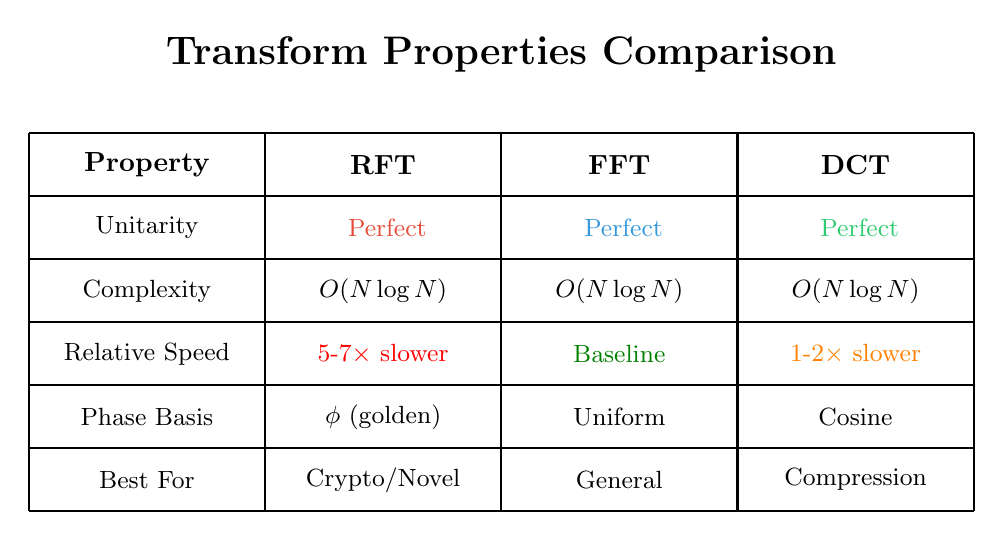
\begin{tikzpicture}
    \node[font=\Large\bfseries] at (6, 0) {Transform Properties Comparison};
    
    \begin{scope}[shift={(0,-1)}]
        % Table
        \draw[thick] (0, 0) -- (12, 0);
        \draw[thick] (0, -0.8) -- (12, -0.8);
        \draw[thick] (0, -1.6) -- (12, -1.6);
        \draw[thick] (0, -2.4) -- (12, -2.4);
        \draw[thick] (0, -3.2) -- (12, -3.2);
        \draw[thick] (0, -4.0) -- (12, -4.0);
        \draw[thick] (0, -4.8) -- (12, -4.8);
        
        % Vertical lines
        \draw[thick] (0, 0) -- (0, -4.8);
        \draw[thick] (3, 0) -- (3, -4.8);
        \draw[thick] (6, 0) -- (6, -4.8);
        \draw[thick] (9, 0) -- (9, -4.8);
        \draw[thick] (12, 0) -- (12, -4.8);
        
        % Headers
        \node[font=\bfseries] at (1.5, -0.4) {Property};
        \node[font=\bfseries] at (4.5, -0.4) {RFT};
        \node[font=\bfseries] at (7.5, -0.4) {FFT};
        \node[font=\bfseries] at (10.5, -0.4) {DCT};
        
        % Row 1: Unitarity
        \node[font=\small] at (1.5, -1.2) {Unitarity};
        \node[font=\small, color=rftcolor] at (4.5, -1.2) {$\checkmark$ Perfect};
        \node[font=\small, color=fftcolor] at (7.5, -1.2) {$\checkmark$ Perfect};
        \node[font=\small, color=dctcolor] at (10.5, -1.2) {$\checkmark$ Perfect};
        
        % Row 2: Complexity
        \node[font=\small] at (1.5, -2.0) {Complexity};
        \node[font=\small] at (4.5, -2.0) {$O(N\log N)$};
        \node[font=\small] at (7.5, -2.0) {$O(N\log N)$};
        \node[font=\small] at (10.5, -2.0) {$O(N\log N)$};
        
        % Row 3: Relative Speed
        \node[font=\small] at (1.5, -2.8) {Relative Speed};
        \node[font=\small, color=red] at (4.5, -2.8) {5-7$\times$ slower};
        \node[font=\small, color=green!50!black] at (7.5, -2.8) {Baseline};
        \node[font=\small, color=orange] at (10.5, -2.8) {1-2$\times$ slower};
        
        % Row 4: Phase Structure
        \node[font=\small] at (1.5, -3.6) {Phase Basis};
        \node[font=\small] at (4.5, -3.6) {$\phi$ (golden)};
        \node[font=\small] at (7.5, -3.6) {Uniform};
        \node[font=\small] at (10.5, -3.6) {Cosine};
        
        % Row 5: Best Use
        \node[font=\small] at (1.5, -4.4) {Best For};
        \node[font=\small] at (4.5, -4.4) {Crypto/Novel};
        \node[font=\small] at (7.5, -4.4) {General};
        \node[font=\small] at (10.5, -4.4) {Compression};
    \end{scope}
\end{tikzpicture}

\vspace{1cm}

%% Figure 6: Mathematical Definition Box
\begin{tikzpicture}
    \node[draw, thick, rounded corners, fill=gray!10, text width=14cm, align=left, font=\small] at (7, 0) {
        \textbf{Φ-RFT Mathematical Definition:}\\[0.3cm]
        \textbf{Forward Transform:}\\
        $\displaystyle Y = D_\phi \circ C_\sigma \circ \text{FFT}(x)$\\[0.2cm]
        Where:
        \begin{itemize}
            \item $D_\phi[k] = e^{i\cdot 2\pi\beta \cdot \text{frac}(k/\phi)}$ \quad (Golden-ratio phase)
            \item $C_\sigma[k] = e^{i\pi\sigma k^2/N}$ \quad (Chirp phase)
            \item $\phi = \frac{1+\sqrt{5}}{2} \approx 1.618$ \quad (Golden ratio)
        \end{itemize}
        \vspace{0.2cm}
        \textbf{Inverse Transform:}\\
        $\displaystyle x = \text{IFFT}(\overline{C_\sigma} \circ \overline{D_\phi} \circ Y)$\\[0.2cm]
        \textbf{Unitarity Condition:}\\
        $\Psi^\dagger \Psi = I$ \quad $\Rightarrow$ \quad $\|\Psi x\|_2 = \|x\|_2$ \quad (Energy preservation)
    };
\end{tikzpicture}

\end{document}
